\documentclass[a5paper]{article}
\usepackage[a5paper, top=8mm, bottom=8mm, left=8mm, right=8mm]{geometry}

\usepackage{polyglossia}
\setdefaultlanguage[babelshorthands=true]{russian}

\usepackage{fontspec}
\setmainfont{FreeSerif}
\newfontfamily{\russianfonttt}[Scale=0.7]{DejaVuSansMono}

\usepackage[font=scriptsize]{caption}

\usepackage{amsmath}
\usepackage{amssymb,amsfonts,textcomp}
\usepackage{color}
\usepackage{array}
\usepackage{hhline}
\usepackage{cite}

\usepackage[hang,multiple]{footmisc}
\renewcommand{\footnotelayout}{\raggedright}

\PassOptionsToPackage{hyphens}{url}\usepackage[xetex,linktocpage=true,plainpages=false,pdfpagelabels=false]{hyperref}
\hypersetup{colorlinks=true, linkcolor=blue, citecolor=blue, filecolor=blue, urlcolor=blue, pdftitle=1, pdfauthor=, pdfsubject=, pdfkeywords=}

\usepackage{tabu}

\usepackage{graphicx}
\usepackage{indentfirst}
\usepackage{multirow}
\usepackage{subfig}
\usepackage{footnote}
\usepackage{minted}

\sloppy
\pagestyle{plain}

\title{ASP.NET MVC Core, демонстрация}
\author{Юрий Литвинов\\\small{yurii.litvinov@gmail.com}}

\date{16.11.2017}

\begin{document}

\maketitle
\thispagestyle{empty}

\section{Создание проекта}

Напишем в качестве демонстрации небольшое приложение, которое позволяет, например, регистрироваться на конференцию. Показывать я буду на примере Visual Studio. Надо, чтобы была установлена ``рабочая нагрузка'' ``ASP.NET и разработка веб-приложений''.

Начнём с создания нового проекта. Visual C\# -> ASP.NET Core Web Application, указываем тип приложения как Web Application (Model-View-Controller), остальные настройки оставляем по умолчанию:

\begin{center}
	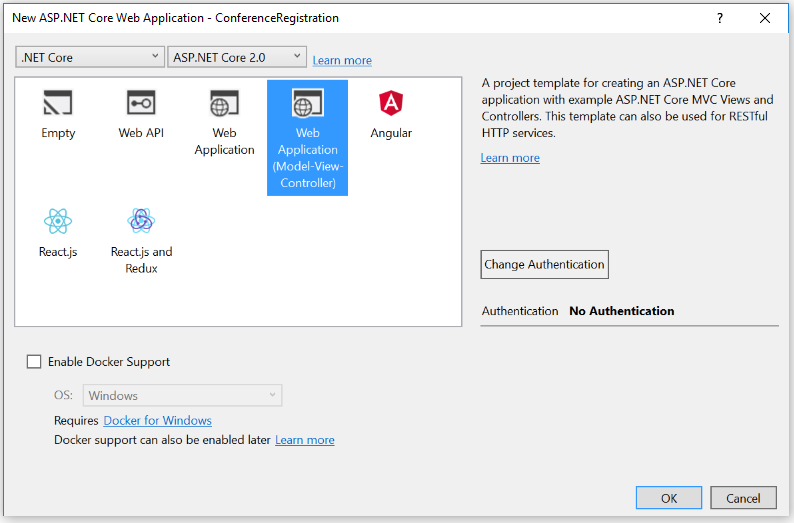
\includegraphics[width=0.7\textwidth]{projectCreation.png}
\end{center}

Стоит отметить, что рекомендованный способ создания веб-приложений под ASP.NET Core 2.0 --- это Razor Pages (в этом диалоге --- просто Web Application), более ``легковесная'' архитектура. Здесь показано полноценное MVC-приложение,
прежде всего потому, что так же точно выглядели приложения в MVC 5 (которая всё ещё очень популярна) и потому, что основные принципы библиотеки в MVC-варианте проще проиллюстрировать.

Сгенерированный из шаблона проект имеет следующую структуру.
\begin{itemize}
	\item \textbf{wwwroot} --- папка со \textit{статическими ресурсами}, то есть файлами, которые можно использовать в своих HTML-страницах, и которые будут отправлены на клиент как они есть.
	\item \textbf{Controllers} --- папка с \textit{контроллерами}, то есть кодом на C\#, обрабатывающим входящие запросы. Обычно один контроллер отвечает сразу за несколько связанных по смыслу запросов,
		в нашем приложении сейчас всего один контроллер с тремя методами, каждый из которых на самом деле вызывается самой MVC, когда приходит запрос на URL, содержащий имя метода контроллера.
	\item \textbf{Models} --- сюда кладутся классы View Model, которые контроллеры будут заполнять и отправлять во View. Сюда же иногда кладут классы Domain Model, классы, обеспечивающие сохранение модели в базу и т.д., и для небольших приложений это даже хорошо работает.
	\item \textbf{Views} --- сюда кладутся .cshtml-файлы, которые представляют собой шаблоны HTML-страниц, используемые Razor-ом для того, чтобы сгенерить представление, которое контроллер потом пошлёт браузеру ответом на запрос. В .cshtml-файлах можно использовать
		данные из моделей, что позволяет параметризовать их полезной информацией в рантайме.
	\item \textbf{appsettings.json} --- конфигурация приложения.
	\item \textbf{bower.json} --- конфигурация пакетов на стороне клиента.
	\item \textbf{bundleconfig.json} --- конфигурация bundling-а и minification-а, используемых для уменьшения времени загрузки страницы путём ужатия её JavaScript-составляющей.
	\item \textbf{Program.cs} --- метод Main, который инициализирует и хостит приложение.
	\item \textbf{Startup.cs} --- конфигурирует MVC-часть приложения --- сервисы и роутинг. Именно тут написано, что если мы просто запустили приложение, то должен вызваться метод Index у контроллера HomeController (обратите внимание, что в роуте он пишется как просто Home, 
		это одно из многих соглашений об именовании, которые используются повсюду в MVC)
\end{itemize}

Запустим и посмотрим, что получилось. Для этого достаточно просто нажать на ``Запустить'', но можно посмотреть на кнопку запуска внимательнее и выяснить, что она позволяет выбрать \textit{хостинг} для нашего приложения и браузер, в котором мы хотим наше приложение посмотреть.
Под виндой для отладки обычно используется IIS Express, который запускается самой Visual Studio, но можно сказать приложению хостить самого себя, тогда будет использоваться веб-сервер Kestrel, запускаемый внутри процесса самого приложения. Приложение запустится в выбранном браузере
по адресу localhost (потому что отладочные серверы по умолчанию извне локального компьютера не видны) и случайному порту, определяемому при запуске (впрочем, это можно перенастроить в свойствах проекта, во вкладке Debug). Ещё обратите внимание, что, в отличие от десктопных приложений,
закрытие окна браузера не всегда означает остановку приложения --- Visual Studio старается делать это сама, следя за процессом браузера, но у неё не всегда получается, и иногда надо останавливать процесс с веб-приложением вручную.

\section{Hello, world}

Начнём с того, что удалим всё, что нагенерилось. Добавим новый контроллер, назовём его так же HomeController, добавим в него метод Index (методы в контроллере, кстати, называются Action), который будет возвращать вид MyView, как-то так:

\begin{minted}{csharp}
using Microsoft.AspNetCore.Mvc;

namespace ConferenceRegistration.Controllers
{
    public class HomeController : Controller
    {
        public IActionResult Index()
        {
            return View("MyView");
        }
    }
}
\end{minted}

Visual Studio справедливо отмечает, что такого вида не существует. Создадим его, Views -> Add..., называем его MyView, говорим, что он должет быть пустой и не использовать лейаут (пока что). Visual Studio всё равно говорит в контроллере, что вида не существует ---
потому что используются умолчания, контроллер ищет все виды, относящиеся к нему, в подпапке папки Views, которая называется так же, как контроллер. Должно получиться как-то так:

\begin{center}
	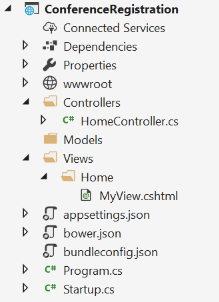
\includegraphics[width=0.45\textwidth]{projectStructure.png}
\end{center}

Ещё раз обратите внимание, что папка называется не HomeController, а Home.

Теперь пойдём в MyView.cshtml, увидим там заглушку с пустой HTML-страницей и начнём верстать HTML как настоящие веб-разработчики:

\begin{minted}{html}
@{
    Layout = null;
}

<!DOCTYPE html>

<html>
<head>
    <meta name="viewport" content="width=device-width" />
    <title>MyView</title>
</head>
<body>
Hello, world!
</body>
</html>
\end{minted}

Получилось хорошо, но для этого не нужен никакой MVC, одной HTML-страницы было бы вполне достаточно. Чтобы было чуть более интересно, давайте показывать текущее время на сервере (на момент запроса, естественно). Для этого надо сначала слегка модифицировать контроллер, чтобы он отправлял
клиенту текущее время:

\begin{minted}{csharp}
public IActionResult Index()
{
    ViewBag.Time = DateTime.Now;
    return View("MyView");
}
\end{minted}

И View:

\begin{minted}{html}
@{
    Layout = null;
}

<!DOCTYPE html>

<html>
<head>
    <meta name="viewport" content="width=device-width" />
    <title>MyView</title>
</head>
<body>
Hello, world! Time is @ViewBag.Time
</body>
</html>
\end{minted}

Выглядит как чёрная магия, но на самом деле довольно просто и удобно. ViewBag --- это dynamic-свойство класса Controller, поэтому в него можно присваивать что угодно и как угодно. Он всегда передаётся View, где Razor может использовать его для генерации HTML-страницы 
(обратите внимание, на клиент отправляется уже готовая HTML-страница, никаких ViewBag-ов там нет). ``@'' в тексте HTML как раз и означает подстановку данных из модели в шаблон (на самом деле, любое выражение на C\#, для него делается ToString() и печатается в HTML). В роли модели у нас тут
выступает ViewBag, что обладает очевидным недостатком --- если мы не угадали с именем полей в контроллере или виде, то узнаем мы об этом только во время выполнения. Поэтому придумали типизированные модели.

\section{Демо-приложение, базовая функциональность}

Итак, мы хотим приложение, позволяющее регистрироваться на конференции. Для этого надо:
\begin{itemize}
	\item Титульную страницу с информацией о конференции и ссылкой на форму регистрации
	\item Саму форму регистрации, которая бы спрашивала имя-фамилию, электронную почту и с докладом/без доклада мы хотим участвовать
	\item Страницу, на которой можно просмотреть всех зарегистрировавшихся
\end{itemize}

Не будем делать авторизацию и подобные вещи, хотя ASP.NET это, конечно умеет. Однако с валидацией на стороне сервера и с оформлением страницы попробуем повозиться.

Начать следует, как и обычно при разработке информационных систем, с модели предметной области. Для больших приложений применяются UML-диаграммы, методы анализа предметной области\footnote{Рекомендую Эрик Эванс, ``Предметно-ориентированное проектирование'' как очень неплохую книжку по этому вопросу},
но для маленьких приложений проще и быстрее выразить свою мысль прямо в коде на C\#. Создадим новый класс в папке Models с вот таким содержимым:

\begin{minted}{csharp}
namespace ConferenceRegistration.Models
{
    public class Participant
    {
        public string Name { get; set; }
        public string Email { get; set; }
        public bool? Speaker { get; set; }
    }
}
\end{minted}

Теперь модифицируем контроллер, добавив в него action, который будет возвращать вид со страницей регистрации, где и можно будет заполнить нашу модель:

\begin{minted}{csharp}
namespace ConferenceRegistration.Controllers
{
    public class HomeController : Controller
    {
        public IActionResult Index()
        {
            ViewBag.Time = DateTime.Now;
            return View("MyView");
        }

        public IActionResult Register()
        {
            return View();
        }
    }
}
\end{minted}

Обратите внимание, что тут мы не передаём в метод View параметр с именем View --- применяется умолчание, которое говорит View искать .cshtml-файл с именем, соответствующим имени метода контроллера (в папке с именем, соответствующем имени самого контроллера).
Соответственно, надо создать этот View:

\begin{center}
	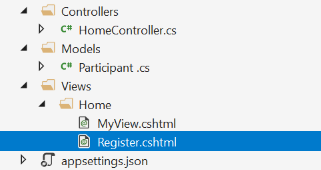
\includegraphics[width=0.4\textwidth]{secondView.png}
\end{center}

Теперь добавим на главную страницу (MyView.cshtml) ссылку на страницу с регистрацией (которая пока пустая) и заодно больше контента:

\begin{minted}{html}
@{
    Layout = null;
}

@addTagHelper *, Microsoft.AspNetCore.Mvc.TagHelpers

<!DOCTYPE html>

<html>
<head>
    <meta name="viewport" content="width=device-width" />
    <title>MyView</title>
</head>
<body>
    <div>
        <p>SEIM-2018 conference will be held on 14th April in St. Petersburg.</p>
        <a asp-action="Register">Register now!</a>
    </div>
</body>
</html>
\end{minted}

Здесь появилась новая концепция, важная для Razor --- так называемый tag helper. Выглядит оно как атрибут тэга HTML, но на самом деле это код на C\#, который может что-то делать с HTML-кодом. В данном случае мы используем библиотечный хелпер asp-action, который
генерирует правильную ссылку на вид, указанный ему в качестве параметра. Это позволяет не хардкодить ссылки на страницы внутри приложения, что облегчает рефакторинг. Существует ещё куча хелперов, подключаются они директивой @addTagHelper и обычно не здесь, а в файле
Views/\_ViewImports.cshtml --- чтобы быть доступными по всему проекту.

Теперь можно наконец накодить форму регистрации:

\begin{minted}{html}
@model ConferenceRegistration.Models.Participant

@addTagHelper *, Microsoft.AspNetCore.Mvc.TagHelpers

@{
    Layout = null;
}

<!DOCTYPE html>

<html>
<head>
    <meta name="viewport" content="width=device-width" />
    <title>Register</title>
</head>
<body>
    <form asp-action="Register" method="post">
        <p>
            <label asp-for="Name">Your name:</label>
            <input asp-for="Name" />
        </p>
        <p>
            <label asp-for="Email">Your email:</label>
            <input asp-for="Email" />
        </p>
        <p>
            <label>Are you a speaker?</label>
            <select asp-for="Speaker">
                <option value="">Choose an option</option>
                <option value="true">Yes</option>
                <option value="false">No</option>
            </select>
        </p>
        <button type="submit">Register!</button>
    </form>
</body>
</html>
\end{minted}

Здесь используется обычная для HTML штука для ввода данных --- форма. Когда пользователь заполняет поля и жмёт на кнопку, помеченную атрибутом type="submit", браузер выполянет POST-запрос, в теле которого на сервер передаются данные из полей формы. Хелпер asp-for генерит дополнительные
HTML-атрибуты, которые позволяют идентифицировать данные и сопоставить их свойствам объекта, указанного в тэге @model. Пока что по клику на Register поля просто очищаются и ничего больше не происходит. 
Дело в том, что запрос шлётся всё к тому же нашему методу Register, который возвращает View с формой, разумеется, пустой.

Чтобы это исправить, возвращаемся в контроллер и используем тот факт, что просто открытие браузером страницы --- это GET-запрос, а отправка заполненной формы --- это POST-запрос, даже если они идут на один адрес. Пишем ещё одно действие в контроллере, которое будет реагировать конкретно
на POST:

\begin{minted}{csharp}
public class HomeController : Controller
{
    public IActionResult Index()
    {
        ViewBag.Time = DateTime.Now;
        return View("MyView");
    }

    [HttpGet]
    public IActionResult Register()
    {
        return View();
    }

    [HttpPost]
    public IActionResult Register(Participant participant)
    {
        // TODO: Do something with registration info
        return View();
    }
}
\end{minted}

Пока что внешне ничего не изменилось, но теперь хотя бы понятно, куда писать содержательную логику. Этим мы сейчас и займёмся. 

Заведём в Models ещё один класс, назовём его Repository. Он будет просто хранить список зарегистрированных пользователей в памяти, что, конечно, не очень хорошо, потому что при перезапуске приложения информация потеряется, но работой с БД мы займёмся чуть позже.
Класс мы сделаем static, потому что, казалось бы, идеологически правильно эту информацию хранить в HomeController, но контроллер создаётся каждый раз заново при обработке запроса, так что там ничего хранить не получится.
Выглядеть наш репозиторий будет так:

\begin{minted}{csharp}
namespace ConferenceRegistration.Models
{
    public static class Repository
    {
        private static readonly IList<Participant> participants = new List<Participant>();

        public static IEnumerable<Participant> Participants => participants;

        public static void AddParticipant(Participant participant) 
            => participants.Add(participant);
    }
}
\end{minted}

Теперь модифицируем контроллер, чтобы он добавлял в него информацию по мере получения её от пользователя:

\begin{minted}{csharp}
public class HomeController : Controller
{
    public IActionResult Index()
    {
        ViewBag.Time = DateTime.Now;
        return View("MyView");
    }

    [HttpGet]
    public IActionResult Register()
    {
        return View();
    }

    [HttpPost]
    public IActionResult Register(Participant participant)
    {
        Repository.AddParticipant(participant);
        return View();
    }
}
\end{minted}

Тут, кстати, должен возникнуть вопрос, почему Register --- это метод, обрабатывающий POST-запрос от браузера, но он принимает параметр типа Participant --- браузер же ничего не знает про C\#-классы. На самом деле парсит информацию от браузера сам MVC, создаёт объект и заполняет его данными
из запроса. Этот механизм называется Model binding, и он достаточно умён, чтобы парсить POST-запросы и даже параметры, передаваемые в адресной строке в GET-запросах.

Давайте ещё сделаем страницу подтверждения регистрации, добавив новый .cshtml в Views/Home:

\begin{minted}{html}
@model ConferenceRegistration.Models.Participant

@{
    Layout = null;
}

<!DOCTYPE html>

<html>
<head>
    <meta name="viewport" content="width=device-width" />
    <title>Thanks</title>
</head>
<body>
<p>
    <h1>Thank you, @Model.Name</h1>
</p>
<p>
    @if (Model.Speaker == true)
    {
        @:Please don't forget to submit your article!
    }
</p>
</body>
</html>
\end{minted}

Тут мы видим, как модель может быть использована даже для условной генерации HTML-кода. Razor интересен тем, что можно просто писать C\#-код, помечая его начало символом ``@'', и он сам догадается, где он заканчивается и начинается HTML.

Ну и последнее, что нам нужно сделать --- это страницу со списком зарегистрировавшихся на конференцию. Начнём с модификации контроллера. Допишем в HomeController метод ListParticipants:
\begin{minted}{csharp}
public IActionResult ListParticipants()
    => View(Repository.Participants);
\end{minted}

А теперь сделаем для него View:

\begin{minted}{html}
@model IEnumerable<ConferenceRegistration.Models.Participant>

@{
    Layout = null;
}

<!DOCTYPE html>

<html>
<head>
    <meta name="viewport" content="width=device-width" />
    <title>ListParticipants</title>
</head>
<body>

<h2>List of conference participants:</h2>
<table>
    <thead>
    <tr>
        <th>Name</th>
        <th>Email</th>
        <th>Is speaker</th>
    </tr>
    </thead>
    <tbody>
    @foreach (ConferenceRegistration.Models.Participant p in Model) {
        <tr>
            <td>@p.Name</td>
            <td>@p.Email</td>
            <td>@(p.Speaker == true ? "Yes" : "No")</td>
        </tr>
    }
    </tbody>
</table>

</body>
</html>
\end{minted}

Было бы логично предоставлять эту информацию только организаторам, поэтому мы не будем делать ссылок на эту страницу (хотя должны были бы сделать авторизацию, но нам слишком лень). Попасть на неё можно, написав в браузере что-то вроде ``http://localhost:49510/Home/ListParticipants''.
Предполагается, что про эту ссылку знают только организаторы.

Запускаем, регистрируем пару участников, открываем страницу со списком, видим, что что-то произошло.

\section{Валидация}

Сейчас зарегистрироваться на конференцию можно, просто тыкнув на Register и ничего не вводя. Давайте добавим валидацию, благо это совсем несложно. Просто модифицируем модель:

\begin{minted}{csharp}
public class Participant
{
    [Required(ErrorMessage = "Please enter your name")]
    public string Name { get; set; }

    [Required(ErrorMessage = "Please enter your email")]
    [RegularExpression(".+\\@.+\\..+", ErrorMessage = "Please enter a valid email address")]
    public string Email { get; set; }

    [Required(ErrorMessage = "Please specify whether you'll be a speaker or just attending")]
    public bool? Speaker { get; set; }
}
\end{minted}

Так выглядит декларативное описание правил корректности данных в модели, которое MVC будет применять каждый раз, когда делает model binding при приёме запроса (кстати, обратите внимание, мы специально сделали Speaker nullable, так что если пользователь ничего не ввёл, там будет null). 
Но само по себе оно ничего интересного не делает, кроме выставления флага IsValid в поле ModelState контроллера, поэтому надо ещё модифицировать контроллер:

\begin{minted}{csharp}
[HttpPost]
public IActionResult Register(Participant participant)
{
    if (ModelState.IsValid)
    {
        Repository.AddParticipant(participant);
        return View("Thanks", participant);
    }

    return View();
}
\end{minted}

Так оно не даёт зарегистрироваться пользователю, не смогшему пройти валидацию, но никакой обратной связи не предоставляет, просто возвращая форму регистрации ещё раз. Модифицируем вид:

\begin{minted}{html}
<form asp-action="Register" method="post">
    <div asp-validation-summary="All"></div>
    <p>
        <label asp-for="Name">Your name:</label>
        <input asp-for="Name"/>
    </p>
    ...
</form>
\end{minted}

Теперь получается что-то такое:

\begin{center}
	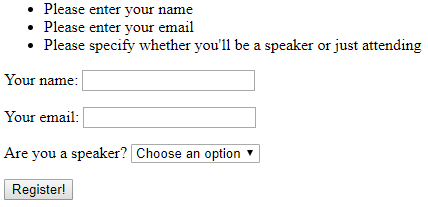
\includegraphics[width=0.6\textwidth]{validationError.png}
\end{center}

Тут мы использовали слишком уж высокоуровневую функциональность для этого туториала (если уж так, то можно было сгенерить форму ввода по модели и вообще ни строчки HTML не писать). И кроме того, такие сообщения об ошибках верификации даже в 90-е годы представить себе трудно, надо 
сделать посимпатичнее. В этом нам поможет тот факт, что хелпер asp-for вставит атрибут class="input-validation-error" в выходной HTML, и мы можем этот класс использовать, чтобы связать с ним стиль отображения элемента, который мы опишем в отдельном .css-файле.

Создаём в папке wwwroot/css новый Style Sheet (например, style.css), пишем туда CSS, который будет управлять внешним видом полей, которые не прошли валидацию:

\begin{minted}{css}
.field-validation-error {
    color: #f00;
}

.field-validation-valid {
    display: none;
}

.input-validation-error {
    border: 1px solid #f00;
    background-color: #fee;
}

.validation-summary-errors {
    font-weight: bold;
    color: #f00;
}

.validation-summary-valid {
    display: none;
}
\end{minted}

Прописываем ссылку на эту .css-ку в форму регистрации:

\begin{minted}{html}
<head>
    <meta name="viewport" content="width=device-width" />
    <title>Register</title>
    <link rel="stylesheet" href="/css/style.css" />
</head>
\end{minted}

Запускаем, получаем форму гораздо симпатичнее:

\begin{center}
	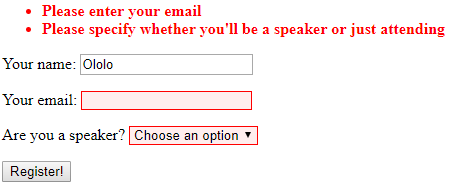
\includegraphics[width=0.6\textwidth]{validationErrorWithCss.png}
\end{center}

\section{Оформление}

Раз уж дело дошло до CSS, можно навести порядок и с оформлением всего сайта. Сейчас он выглядит так, как даже школьники сайты не верстают, поэтому воспользуемся одной из библиотек, доступных в проекте ``из коробки'' --- Bootstrap. Это третьесторонняя опенсорсная библиотека 
(\url{http://getbootstrap.com/}), очень известная в мире веб-разработки, она поставляется вместе с ASP.NET и даже включена в стандартный шаблон MVC-приложения. Bootstrap много чего умеет, но мы воспользуемся некоторыми CSS-стилями, которые она определяет. Например, модифицируем
стартовую страницу так:

\begin{minted}{html}
@{
    Layout = null;
}

@addTagHelper *, Microsoft.AspNetCore.Mvc.TagHelpers

<!DOCTYPE html>

<html>
<head>
    <meta name="viewport" content="width=device-width" />
    <title>Index</title>
    <link rel="stylesheet" href="/lib/bootstrap/dist/css/bootstrap.css" />
</head>
<body>
    <div class="text-center">
        <h3>SEIM-2018 conference will be held on 14th April in St. Petersburg.</h3>
        <a class="btn btn-primary" asp-action="Register">Register now!</a>
    </div>
</body>
</html>
\end{minted}

Добавилось подключение bootstrap.css, атрибуты class="text-center" и class="btn btn-primary", ещё по мелочи изменено внешнее представление. Если сейчас запустить приложение, будет видно, что стало лучше (не то чтобы сильно лучше, но верстаем как можем).

Форма регистрации:

\begin{minted}{html}
@model ConferenceRegistration.Models.Participant

@addTagHelper *, Microsoft.AspNetCore.Mvc.TagHelpers

@{
    Layout = null;
}

<!DOCTYPE html>

<html>
<head>
    <meta name="viewport" content="width=device-width" />
    <title>Register</title>
    <link rel="stylesheet" href="/css/style.css" />
    <link rel="stylesheet" href="/lib/bootstrap/dist/css/bootstrap.css" />
</head>
<body>
<div class="panel panel-success">
    <div class="panel-heading text-center"><h4>Registration form</h4></div>
    <div class="panel-body">
        <form asp-action="Register" method="post">
            <div asp-validation-summary="All"></div>
            <div class="form-group">
                <label asp-for="Name">Your name:</label>
                <input asp-for="Name"/>
            </div>
            <div class="form-group">
                <label asp-for="Email">Your email:</label>
                <input asp-for="Email"/>
            </div>
            <div class="form-group">
                <label>Are you a speaker?</label>
                <select class="form-control" asp-for="Speaker">
                    <option value="">Choose an option</option>
                    <option value="true">Yes</option>
                    <option value="false">No</option>
                </select>
            </div>
            <div class="text-center">
                <button class="btn bg-primary" type="submit">Register!</button>
            </div>
        </form>
    </div>
</div>
</body>
</html>
\end{minted}

Каждому контролу на форме добавились атрибуты class="form-group" и парочка новых div-ов, чтобы повесить на них классы, которые bootstrap будет использовать, чтобы применить стили. Вот что должно было получиться:

\begin{center}
	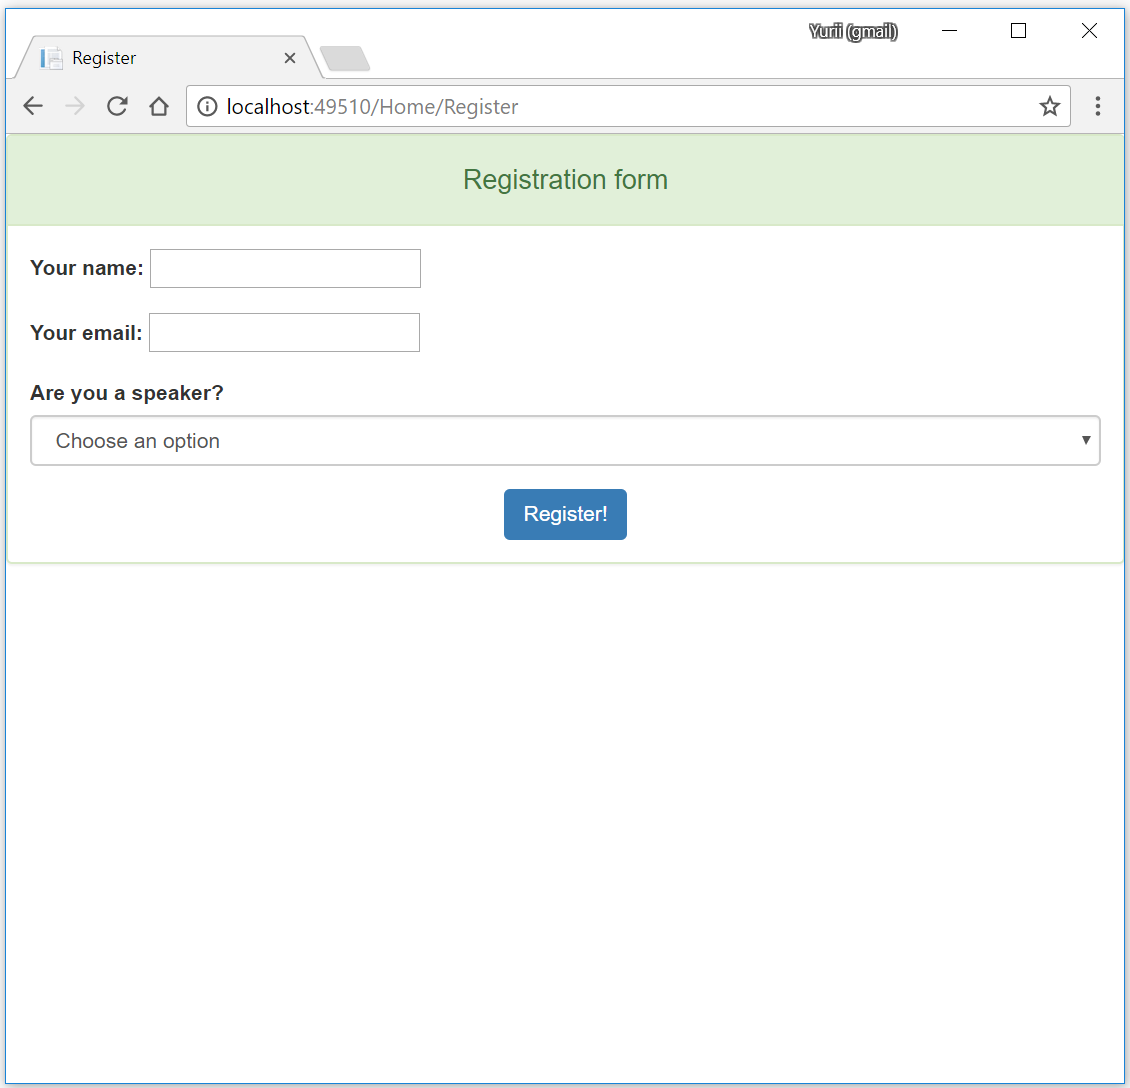
\includegraphics[width=0.6\textwidth]{styledRegisterForm.png}
\end{center}

В целом, наверное, неплохо выглядит на мобильниках. Теперь займёмся страницей со списком участников:

\begin{minted}{html}
@model IEnumerable<ConferenceRegistration.Models.Participant>
@{
    Layout = null;
}
<!DOCTYPE html>
<html>
<head>
    <meta name="viewport" content="width=device-width" />
    <title>ListParticipants</title>
    <link rel="stylesheet" href="/lib/bootstrap/dist/css/bootstrap.css" />
</head>
<body>
    <div class="panel-body">
        <h2>List of conference participants:</h2>
        <table class="table table-striped table-bordered">
            <thead>
                <tr>
                    <th>Name</th>
                    <th>Email</th>
                    <th>Is speaker</th>
                </tr>
            </thead>
            <tbody>
                @foreach (ConferenceRegistration.Models.Participant p in Model)
                {
                    <tr>
                        <td>@p.Name</td>
                        <td>@p.Email</td>
                        <td>@(p.Speaker == true ? "Yes" : "No")</td>
                    </tr>
                }
            </tbody>
        </table>
    </div>
</body>
</html>
\end{minted}

Получилось вот так:

\begin{center}
	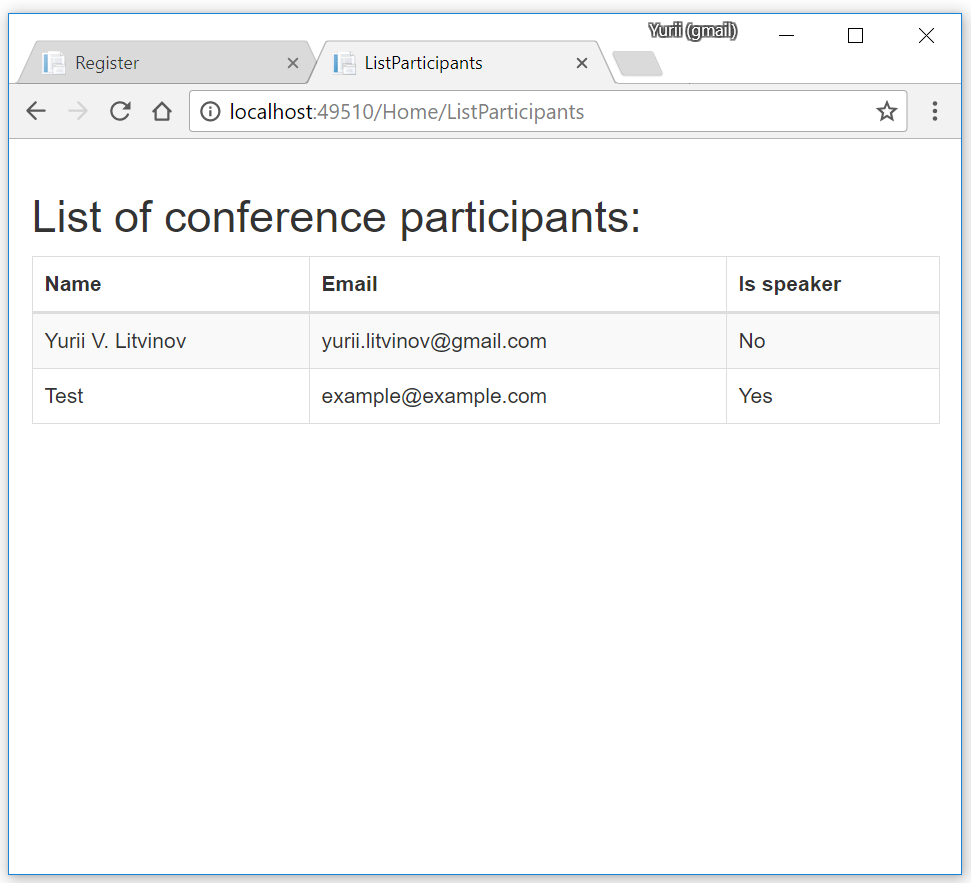
\includegraphics[width=0.55\textwidth]{styledListParticipants.png}
\end{center}

Оформление страницы с подтверждением регистрации оставляется как упражнение.

\section{Добавим персистентность}

Сейчас перезапуск приложения приводит к полной потере данных, что, наверное, не очень, особенно с учётом того, что когда именно приложение решит закрыться --- решать не вам (сервер может решить, что давно не было к нему обращений и прекратить работать). Поэтому воспользуемся
Entity Framework + LocalDB.

Для начала модифицируем наш репозиторий, унаследовав его от DbContext (базового класса из библиотеки Entity Framework, представляющего абстракцию сессии работы с базой):

\begin{scriptsize}
	\begin{minted}{csharp}
public class Repository : DbContext
{
    public DbSet<Participant> Participants { get; set; }

    protected override void OnConfiguring(DbContextOptionsBuilder optionsBuilder)
    {
        optionsBuilder.UseSqlServer(@"Server=(localdb)\mssqllocaldb;Database=ConferenceRegistration;Trusted_Connection=True;");
    }
}
	\end{minted}
\end{scriptsize}

Тут мы захардкодили Connection String, которая содержит информацию о том, как программе связаться с базой. В любом нормальном приложении connection string выносится в конфиг, но для демонстрации сгодится и так. Собственно, 
\begin{verbatim}
	"Server=(localdb)\\\\MSSQLLocalDB;"
\end{verbatim} 
--- это имя драйвера базы данных плюс имя экземпляра сервера, дальше имя базы, которая будет создана на сервере, когда мы начнём работать, дальше настройки подключения. Для каждой СУБД connection string своя, так что надо гуглить, как подключаться к вашей любимой базе.

Дальше модифицируем контроллер, чтобы он работал с новым репозиторием:

\begin{minted}{csharp}
public class HomeController : Controller
{
    public IActionResult Index()
    {
        ViewBag.Time = DateTime.Now;
        return View("MyView");
    }

    [HttpGet]
    public IActionResult Register()
    {
        return View();
    }

    [HttpPost]
    public IActionResult Register(Participant participant)
    {
        if (ModelState.IsValid)
        {
            using (var repository = new Repository())
            {
                repository.Participants.Add(participant);
                repository.SaveChanges();
            }
            return View("Thanks", participant);
        }

        return View();
    }

    public IActionResult ListParticipants()
    {
        using (var repository = new Repository())
        {
            return View(repository.Participants.ToList());
        }
    }
}
\end{minted}

Теперь надо модифицировать модель, добавив атрибут Key свойству, которое мы хотели бы использовать как primary key в базе данных:

\begin{minted}{csharp}
public class Participant
{
    [Required(ErrorMessage = "Please enter your name")]
    public string Name { get; set; }

    [Required(ErrorMessage = "Please enter your email")]
    [RegularExpression(".+\\@.+\\..+", ErrorMessage = "Please enter a valid email address")]
    [Key]
    public string Email { get; set; }

    [Required(ErrorMessage = "Please specify whether you'll be a speaker or just attending")]
    public bool? Speaker { get; set; }
}
\end{minted}

А дальше нам надо поднять экземпляр сервера, создать на нём базу данных, создать в ней таблицу, но... Entity Framework всё сделает за нас с использованием механизма, который называется Migrations. Надо открыть NuGet Manager Console (меню Tools -> NuGet Package Manager -> Package Manager Console) и
написать там Add-Migration Initial. Оно немного подумает и сгенерит папку Migrations в проекте, где будет написано, что надо сделать с базой. А теперь применим миграцию командой Update-Database. Оно ещё немного подумает и напишет, что всё ок, даже ни разу не спросив нас Connection String 
или что-нибудь ещё.

Проверим, что реально что-то произошло. Идём во вкладку Server Explorer, жмём Connect to Database:

\begin{center}
	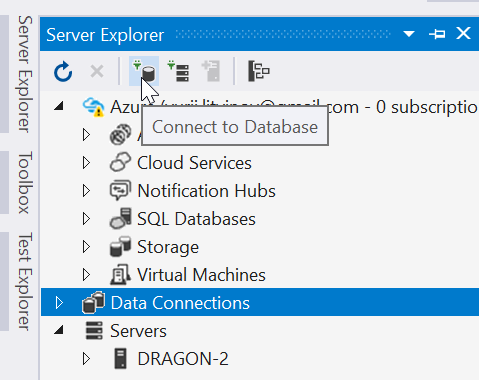
\includegraphics[width=0.45\textwidth]{serverExplorer.png}
\end{center}

В появившемся окне указываем имя сервера и базы, как было в Connection String, так:

\begin{center}
	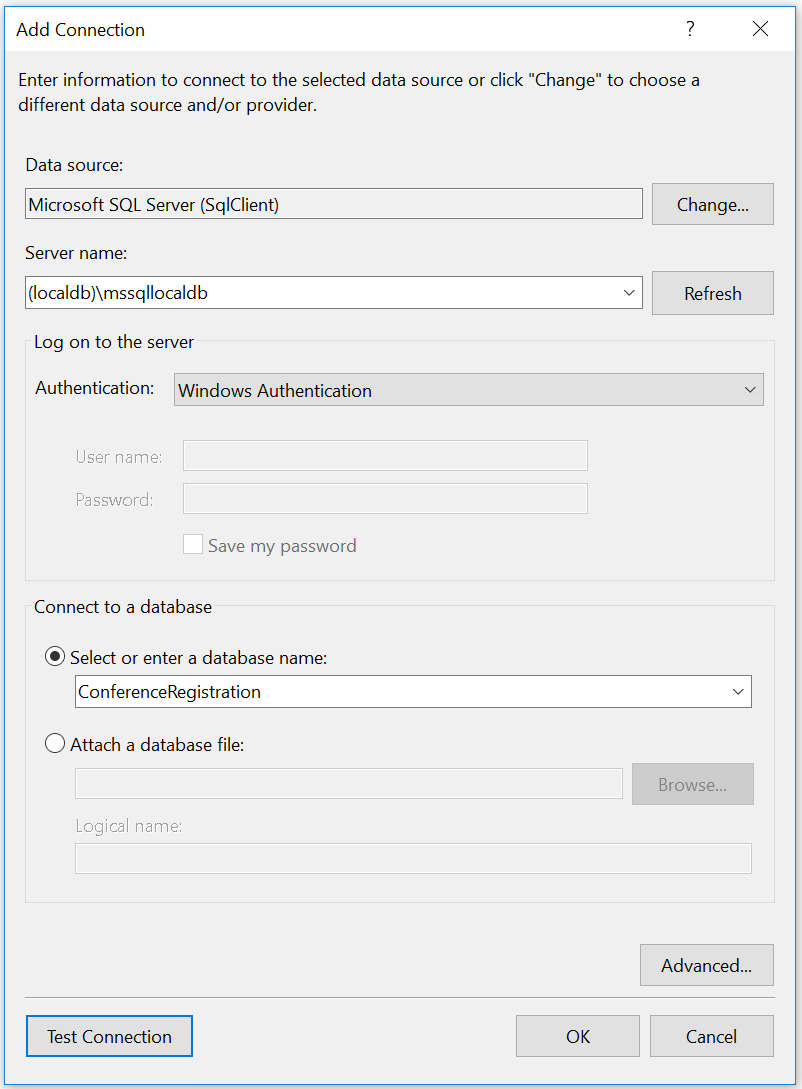
\includegraphics[width=0.65\textwidth]{addConnection.png}
\end{center}

Жмём на Test Connection, если всё ок, жмём на Ок. Теперь содержимое базы можно просмотреть прямо в самой Visual Studio через Server Explorer, как-то так:

\begin{center}
	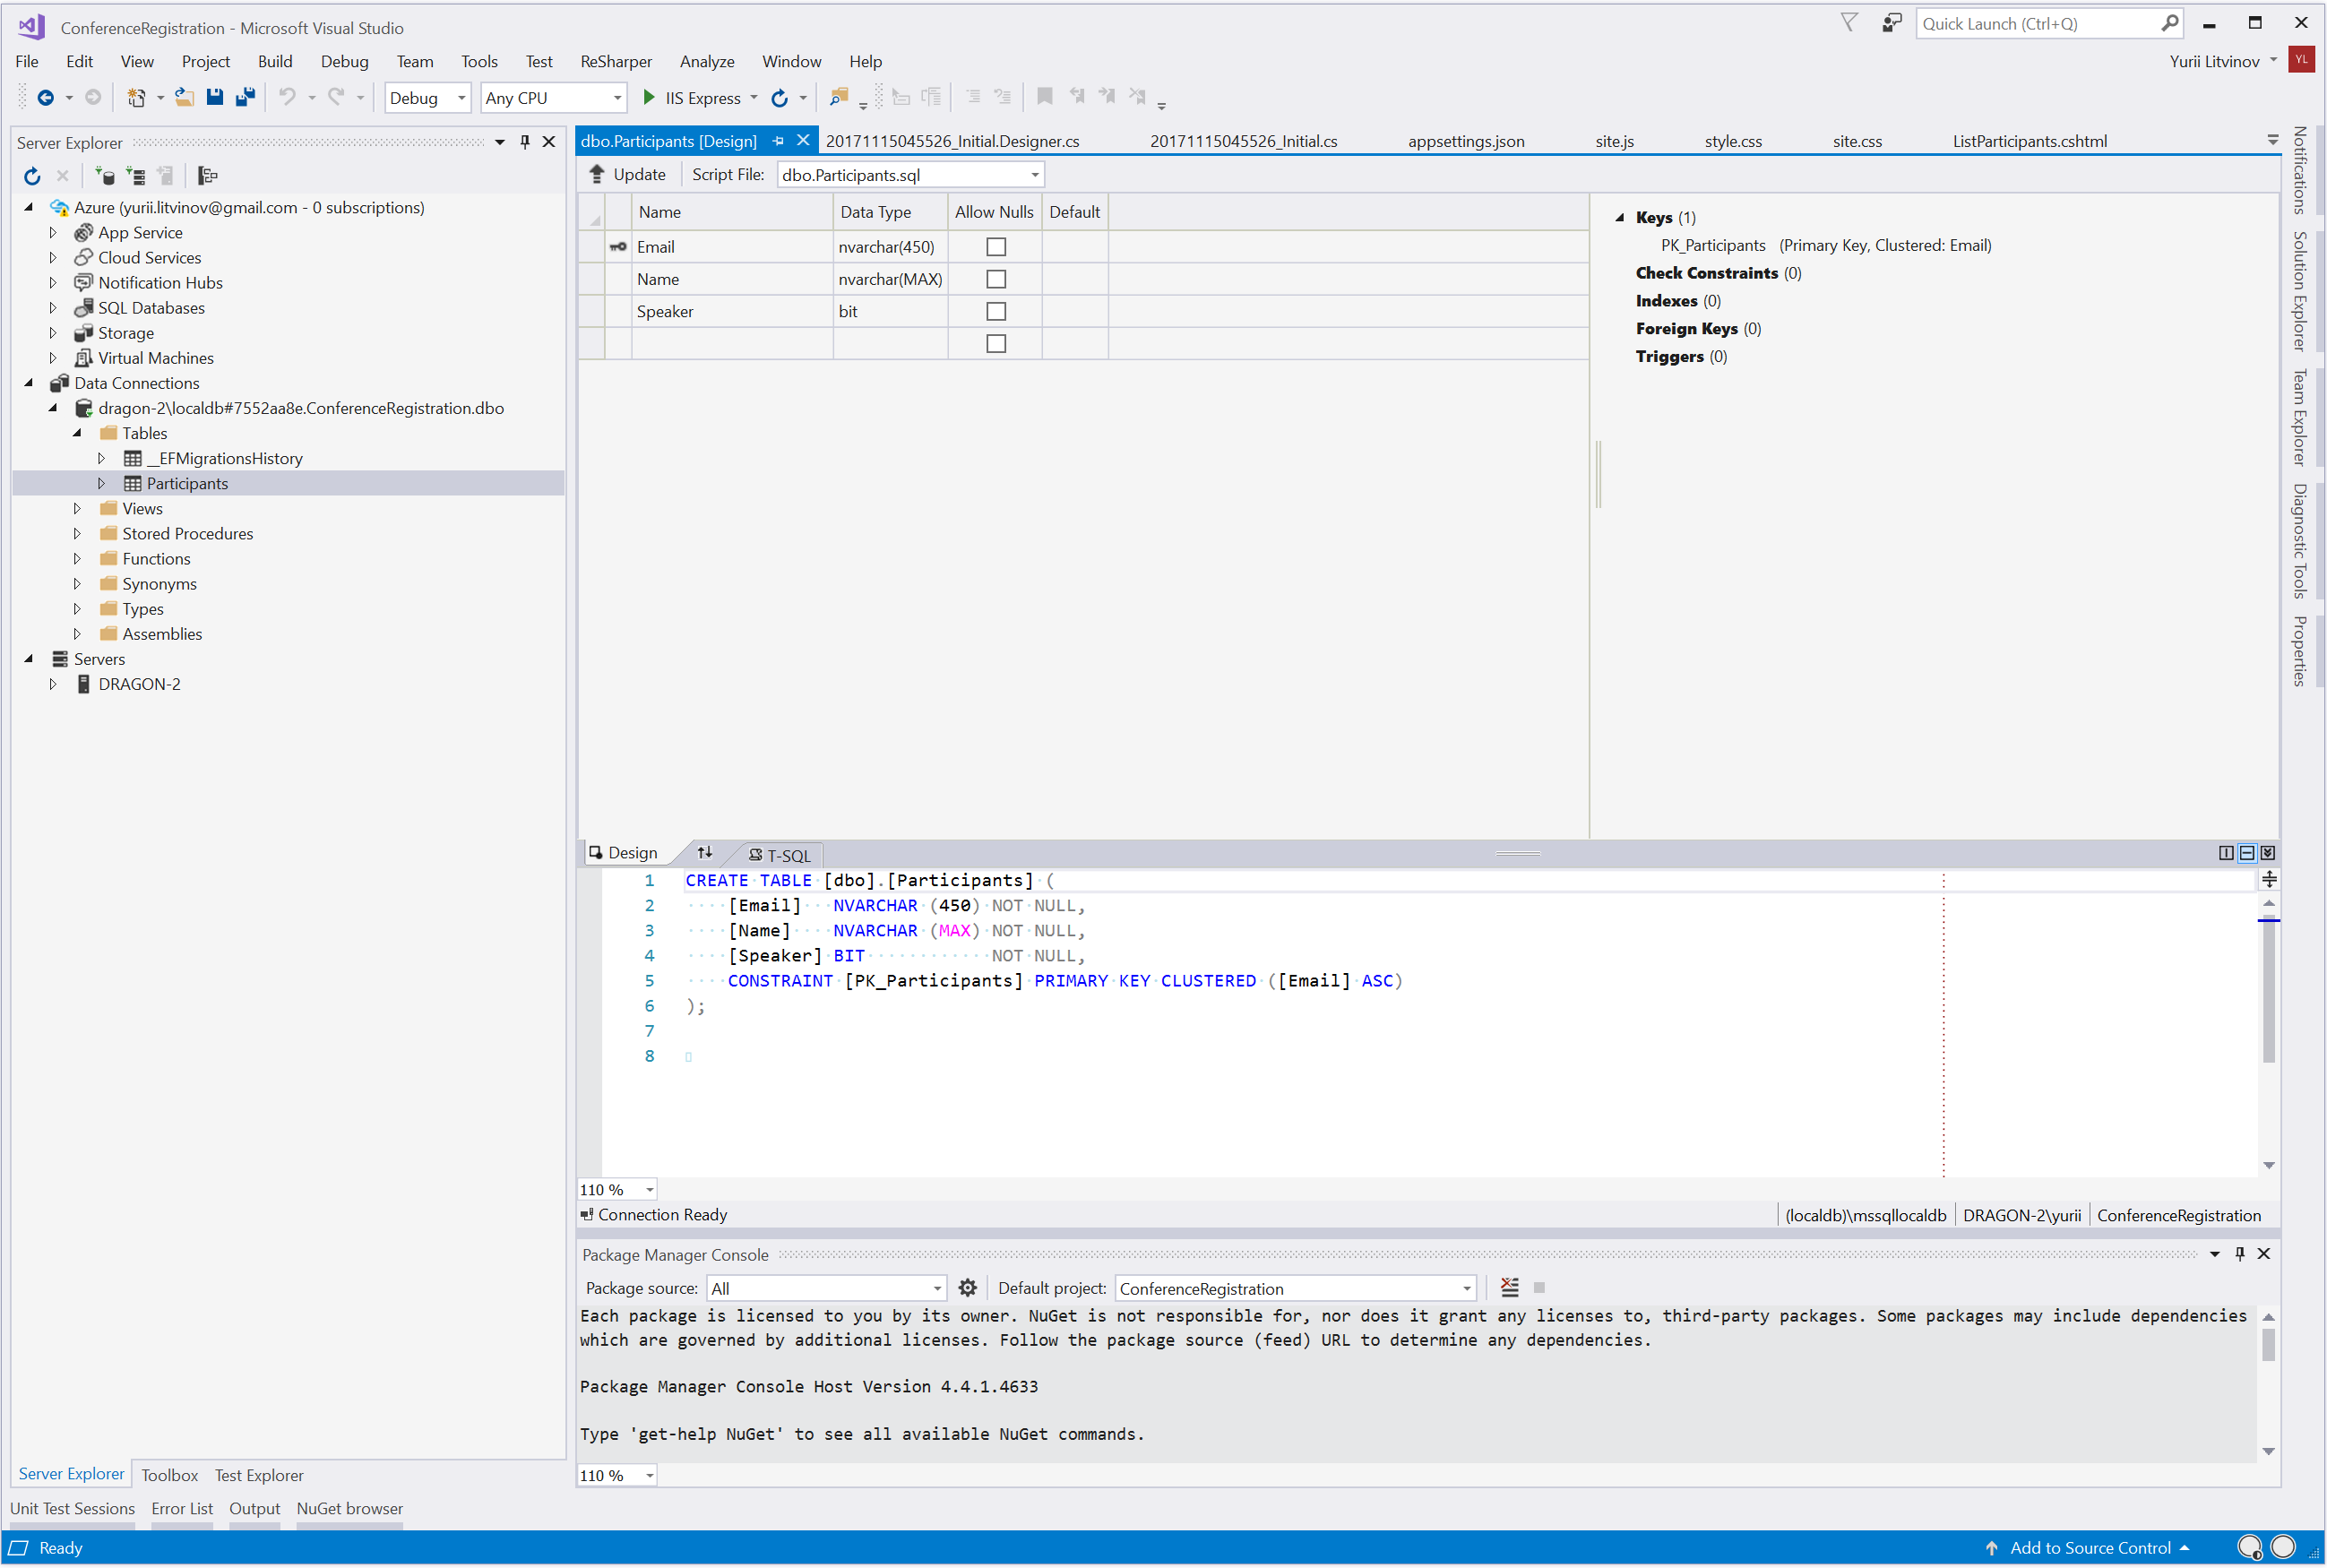
\includegraphics[width=\textwidth]{databaseView.png}
\end{center}

Видим, что там действительно то, что нужно.

Теперь можно запустить приложение, попробовать зарегистрироваться в базе, выключить приложение, выключить сервер (с помощью иконки в трее), заново запустить приложение, и открыв ссылку localhost:<номер порта>/Home/ListParticipants убедиться, что оно реально работает.
Ну а потом грохнуть базу через Server Explorer, если она больше не нужна.

\end{document}
